%
% uaThesis example (for a thesis written in Portuguese)
%
% the complete list of options and commands can be found in uaThesis.sty
%

\documentclass[11pt,twoside,a4paper]{report}
\usepackage[utf8]{inputenc}
\usepackage[DETI,newLogo]{uaThesis}

\def\ThesisYear{2023}

% optional packages
\usepackage[english]{babel}
\usepackage{hyperref}
\usepackage{amsmath}
\usepackage{amssymb}
\usepackage{xspace}% used by \sigla
\usepackage{listings}
\usepackage{multicol}
\usepackage{graphicx}
\usepackage[acronym]{glossaries}


% optional (comment to use default)s
%   depth of the table of contents
%     1 ... chapther and sections
%     2 ... chapters, sections, and subsections
%     3 ... chapters, sections, subsections, and subsubsections
\setcounter{tocdepth}{3}

% optional (comment to used default)
%   horizontal line to separate floats (figures and tables) from text
\def\topfigrule{\kern 7.8pt \hrule width\textwidth\kern -8.2pt\relax}
\def\dblfigrule{\kern 7.8pt \hrule width\textwidth\kern -8.2pt\relax}
\def\botfigrule{\kern -7.8pt \hrule width\textwidth\kern 8.2pt\relax}

% custom macros (could also be defined using \newcommand)
\def\I{\mathtt{i}}         % one possible way to represent $\sqrt{-1}$
\def\Exp#1{e^{2\pi\I #1}}  % argument inside braces, i.e., "{}"
\def\EXP#1.{e^{2\pi\I #1}} % argument finishes when a full stop is encountered, i.e., "."
\def\sigla{\LaTeX\xspace}  % use as "blabla \sigla blabla (no need to do "blabla \sigla\ blabla"

\def\AddVMargin#1{\setbox0=\hbox{#1}%
                  \dimen0=\ht0\advance\dimen0 by 2pt\ht0=\dimen0%
                  \dimen0=\dp0\advance\dimen0 by 2pt\dp0=\dimen0%
                  \box0}   % add extra vertical space above and below the argument (#1)
\def\Header#1#2{\setbox1=\hbox{#1}\setbox2=\hbox{#2}%
           \ifdim\wd1>\wd2\dimen0=\wd1\else\dimen0=\wd2\fi%
           \AddVMargin{\parbox{\dimen0}{\centering #1\\#2}}} % put #1 on top #2


\makeglossaries

%
% Acronyms
%
\newacronym{ua}{UA}{University of Aveiro}
\newacronym{vpn}{VPN}{Virtual Private Network}
\newacronym{iris}{IRIS-Lab}{Intelligent Robotics and Systems Laboratory}
\newacronym{p2p}{P2P}{Peer to Peer}
\newacronym{ros}{ROS}{Robot Operating System}
\newacronym{rtt}{RTT}{Round Trip Time}
\newacronym{ddos}{DDOS}{Distributed Denial Of Service}
\newacronym{oor}{OOR}{Open Overlay Router}
\newacronym{nat}{NAT}{Network Address Translator}
\newacronym{sa}{SA}{Security Association}
\newacronym{ah}{AH}{Authentication Header}
\newacronym{esp}{ESP}{Encapsulating Security Payload}
\newacronym{spi}{SPI}{Security Parameter Index}
\newacronym{ike}{IKE}{Internet Key Exchange}
\newacronym{icv}{ICV}{Integrity Check Value}
\newacronym{ssl}{SSL}{Secure Sockets Layer}
\newacronym{DERP}{DERP}{Designated Encrypted Relay for Packets}
\newacronym{stun}{STUN}{Session Traversal Utilities for NAT}
\newacronym{edm}{EDM}{Endpoint-Dependent Mapping}
\newacronym{eim}{EIM}{Endpoint-Independent Mapping}
\newacronym{http}{HTTP}{Hyper-Text Transfer Protocol}


\begin{document}

%
% Cover page (use only one of the first two \TitlePage)
%

%
% Initial thesis pages
%

\TitlePage
  \HEADER{\BAR\FIG{\begin{minipage}{50mm} % no more than 120mm
          ``An idiot admires complexity, a genius admires simplicity.''
           \begin{flushright}
            --- Terry A. Davis
           \end{flushright}
          \end{minipage}}}
         {\ThesisYear}
  \TITLE{Vasco Regal Sousa}
        {Multiple Client Wireguard Based Private and Secure Overlay Network}
\EndTitlePage
\titlepage\ \endtitlepage % empty page

\TitlePage
  \vspace*{55mm}
  \TEXT{\textbf{o j\'uri~/~the jury\newline}}
       {}
  \TEXT{presidente~/~president}
       {\textbf{ABC}\newline {\small
        Professor Catedr\'atico da Universidade de Aveiro (por delega\c c\~ao da Reitora da
        Universidade de Aveiro)}}
  \vspace*{5mm}
  \TEXT{vogais~/~examiners committee}
       {\textbf{DEF}\newline {\small
        Professor Catedr\'atico da Universidade de Aveiro (orientador)}}
  \vspace*{5mm}
  \TEXT{}
       {\textbf{GHI}\newline {\small
        Professor associado da Universidade J (co-orientador)}}
  \vspace*{5mm}
  \TEXT{}
       {\textbf{KLM}\newline {\small
        Professor Catedr\'atico da Universidade N}}
\EndTitlePage
\titlepage\ \endtitlepage % empty page

\TitlePage
  \vspace*{55mm}
  \TEXT{\textbf{agradecimentos~/\newline acknowledgements}}
       {\'Agradecimento especial aos meus gatos}
  \TEXT{}
       {Desejo tamb\'em pedir desculpa a todos que tiveram de suportar o meu desinteresse pelas
        tarefas mundanas do dia-a-dia}
\EndTitlePage
\titlepage\ \endtitlepage % empty page


\TitlePage
  \vspace*{55mm}
  \TEXT{\textbf{Abstract}}
       {An overlay network is a group of computational nodes that communicate with each other through a virtual or logic channel, built on top of another network. Although there are already numerous services and protocols implementing this mechanic, scalibility and administration agility are among the most desired characteristics of such a network topology. Hence, this document presents a centralized solution for the creation and control of secure overlay networks for multiple nodes - from client management to operation auditing, based on Wireguard, an open-source protocol for encrypted communication. In the University of Aveiro, namely the autonomous robot ecosystem residing in the IRIS lab, supporting such a networking architecture would prove to be particular interesting, both for development and project organization.}
\EndTitlePage
\titlepage\ \endtitlepage % empty page


%
% Tables of contents, of figures, ...
%
\pagenumbering{roman}
\tableofcontents

\cleardoublepage
\listoffigures

\cleardoublepage
\listoftables

\cleardoublepage
% \printglossary[type=\acronymtype]

% The chapters (usually written using the isolatin font encoding ...)

\cleardoublepage
\pagenumbering{arabic}
\chapter{Introduction}

\section{Motivation}

Network security has become a topic of evergrowing interest among any information system. Companies strive to ensure their communications follow principles of integrity and confidentially while minimizing attack vectors that could compromise services and data. With such goals in mind, network topologies are subjected to policies which apply rules and conditions to inbound and outbound traffic. One such mechanism is the use of \acrfull{vpn} .

Traditional \acrshort{vpn} services consist in the establishment of a secure, encrypted channel between a client and a network, through an insecure communication medium.


The \acrfull{ua}'s \acrfull{iris} conducts research projects using autonomous mobile robots, which communicate through a Wi-Fi network. Currently, this network is confined to the premises of the \acrshort{iris}, preventing the robots from operating in the remaining \acrshort{ua}'s buildings. Although the \acrshort{ua}'s Wi-Fi infrastructure covers most of its edifices, which can be used by the robots, due to security mechanisms, this network proves to be highly restraining, not allowing \acrfull{p2p} communications through the \acrfull{ros} ~\cite{quigley2009ros} - the operating system the robots run on - middleware without additional network equipments. Moreover, these constraints keep developers from being able to interact with the robots through their personal machines, which, if otherwise possible, would be of great interest.

\section{Objectives}

The main goal of this dissertation is to implement a private overlay network manager to be used exclusively by \acrshort{ua}'s clients. The concept of a manager entails both the definition of a network's client universe (which nodes should be allowed to connect to a certain network) and its respective identification and authentication mechanisms.

In the \acrshort{iris} scenario, the management platform should provide operations to achieve communication between a team of robots, regardless of their physical location within the campus. Moreover, the authentication and connection to a desired overlay network by the robots must be a seemingless operation, requiring little to no manual configuration.

Finally, all traffic must be encrypted and properly authenticated, to ensure the privacy of the communication.

\section{Document Structure}

This document presents an implementation proposal of such an overlay network manager. Hence, it is structured in two main chapters - State of The Art and Methodology. The former consists in an exploration of the background and current state of the art, providing an analysis not only of potential tools, protocols and frameworks suitable for the scope of the dissertation but also of published research conducted covering similar topics and scenarios while the latter establishes the work methodology to be taken for the development and results gathering process.


\cleardoublepage


\chapter{State of the Art}
\label{chapter:sota}

\begin{minipage}{50mm}
     \centering % no more than 120mm
     ``Observation is a dying art''
          \begin{flushright}
          --- Stanley Kubrick
          \end{flushright}
     \end{minipage}

\section{Encrypted Peer to Peer Communications / VPNs}

\acrshort{vpn}s have become a mature technology, with widespread usage among the Internet. With such a range of products offering \acrshort{vpn} capabilities, this section aims to analyze some of its most notable providers, focusing on the processes involved on their respective data planes - which refers to the subsection of a network communication responsible for carrying data between devices. This implies not only the quality of its authentication methods, encryption suite and protocol security but also of its features regarding concepts such as mobility - how the service behaves when clients change their physical locations and IP adresses - and overcoming constraints associated with networks using \acrshort{nat} mechanisms and secured with firewall rules. Finally, since operations taken in the data plane are necessarily associated with a computation overhead, namely traffic encryption and session management, overall performance is also perceived as a valued dimension.

\acrshort{vpn}s can be classified according to their topology in two main categories, client-to-site and site-to-site. A client-to-site \acrshort{vpn} is characterized by connections from a single user (client) to a private network (site), while site-to-site \acrshort{vpn}s offer a secured connection between two private networks. Thus, in site-to-site networks, users are not required to individually configure \acrshort{vpn} clients. The tunnel in this type of \acrshort{vpn} is made available to the entire network.

For the scope of the scenario at hand, where robots (the clients) require access to a private network, there's an emphasis on client-to-site use cases.

\subsubsection{The problem with NAT}

\acrfull{nat} is a networking mechanism responsible for translating IP addresses in private networks into public addresses when packets sent from a private network are routed to the public Internet. In the context of \acrshort{vpn} communications, this process can prove to be a major constraint, not only due to \acrshort{nat}'s tampering of IP packets' fields - namely destination and source addresses - which could potentially compromise its integrity in the eyes of a \acrshort{vpn} protocol, but also regarding the dynamically changing public IP addresses which \acrshort{nat} decides to translate private addresses to.

In fact, it is very likely that devices on the internet reside in a network behind both \acrshort{nat} mechanisms and Firewall rules, with no open ports. Also, believing nodes will have a consistent static IP is a very naive assumption, specially when considering mobile devices. NAT Traversal is a networking technique that enables the establishing and maintaining (by keeping \acrshort{nat} holes open) of \acrshort{p2p} connections between two peers, no matter what's standing between them, making communication possible without the need for firewall configurations or public-facing open ports. There's no one solution to achieve this functionality. In fact, there are various developments effectively implementing a NAT Traversal solution, such as ICE ~\cite{rfc8445} and STUN ~\cite{rfc8489}. Hence, each \acrshort{vpn} service can have its own way of supporting NAT Traversal. Each case is explored seperatly in its own subsection.

\subsection{IPSec}

IPSec refers to an aggregation of layer 3 protocols that work together to create a security extension to the IP protocol by adding packet encryption and authentication. Conceptually, IPSec presents two main dimensions: the protocol defining the transmitted packets' format, when secuirty mechanisms are applied upon them, and the protocol defining how parties in a communication negotiate encryption parameters.

Communication in an IPSec connection is managed according to \acrlong{sa}s (SA). A \acrshort{sa} is an unidirectional set of rules and parameters specifying the necessary information for a secure communication to take place ~\cite{rfc4301}. Here, unidirectional means a \acrshort{sa} can only be associated to either inbound or outbound traffic, but never to both. Hence, an IPSec bidirectional association implies the establishment of two \acrshort{sa} - one for incoming packets and one for outgoing. \acrshort{sa}s specify which security mechanism to use - either \acrfull{ah} or \acrfull{esp} - and are identified by a numeric value, the \acrfull{spi}. Although \acrshort{sa}s can be manually installed in routers, gateways or machines, it becomes impractical as more clients appear. \acrfull{ike} ~\cite{rfc7296} is a negotation protocol which tackles the problems associated with manual \acrshort{sa} installation. In fact, \acrshort{ike} allows the negotation of \acrshort{sa} pairs between any two machines through the use of asymmetric keys or shared secrets.

\subsubsection{Transport and Tunnel modes}

IPsec supports two distinct modes of functionality: transport and tunnel ~\cite{rfc4301}, which differ in the way traffic is dealt with and processed. In the context of \acrshort{vpn}s, tunnel mode presents the
most desirable characteristics. First, tunnel mode encapsulates the original IP packet, allowing the use of private IP addresses as source or destination. Tunnel mode creates the concept of an "outer" and "inner" IP header. The former contains the addresses of the IPSec peers, while the latter contains the real source and destination addresses. Moreover, this very same encapsulation adds confidentiality to the original addresses.

Transport mode requires less computational resources and, consequently, carries less protocol overhead. It does not, however, provide much security compared to tunnel mode, so, in the context of \acrshort{vpn}s, tunnel mode's total protection and confidentiality of the encapsulated IP packet carries much more valuable functionalities.

\subsubsection{Authentication Header}

\acrfull{ah} is a protocol in the IPSec suite providing data origin validation and data integrity consisting in the generation of a checksum via a digest algorithm ~\cite{rfc4302}. Additionally, besides the actual message under integrity check, two other parameters are used under the \acrshort{ah} mechanism. First, to ensure the message was sent from a valid origin, \acrshort{ah} includes a secret shared key. Then, to ensure replay protection, it also includes a sequence number. This last feature consists in the increment, by the sender, of a sequence integer whenever an outgoing message is processed.

\acrshort{ah}, as the name suggests, operates by attaching an header to the IP packets, containing the message's \acrshort{spi}, its sequence number, and the \acrfull{icv} value. This last field is then verified by receivers, which calculate the packet's \acrshort{icv} on their end. The packet is only considered valid if there's a match between the sender and receiver's \acrshort{icv}.

Where this header is inserted depends on the mode IPSec is running. In transport mode, the \acrshort{ah} appears after the IP header and before any next layer protocol or other IPSec headers. As for tunnel mode, the \acrshort{ah} is injected right after the outer IP header.

To calculate the \acrshort{icv}, the \acrshort{ah} requires the value of the source and destination addresses, which raises an incompatibility when faced with networks operating with \acrshort{nat} mechanisms ~\cite{frankel2005guide}.

\subsubsection{Encapsulating Security Payload}

The \acrshort{esp} protocol also offers authentication, integrity and replay protection mechanisms. It differs from \acrshort{ah} by also providing encryption functionalities, where peers in a communication use a shared key for cryptographic operations. Analogous to the previous protocol, the \acrshort{esp}'s header location differs in different IPSec modes. In transport mode, the header is inserted right after the IP header of the original packet. Also, in this mode, since the original IP header is not encrypted, endpoint addresses are visible and might be exposed. As for tunnel mode, a new IP header is created, followed by the \acrshort{esp} header.

Tunnel mode \acrshort{esp} is the most commonly used IPSec mode. This setup not only offers original IP address encryption, concealing source and destination addresses but also supports the adding of padding to packets, difficulting cipher analysis techniques. Moreover, it can be made compatible with \acrshort{nat} and employ \acrshort{nat}-traversal techniques ~\cite{nam2022high}, ~\cite{singh2012nat}.

\subsection{OpenVPN}

OpenVPN ~\cite{ovpnwebsite} is yet another open-source \acrshort{vpn} provider, known for its portability among the most common operating systems due to its user-space implementation. OpenVPN uses established technologies, such as \acrshort{ssl} and asymmetric keys for negotation and authentication and IPSec's \acrshort{esp} protocol, explored in the previous section, over UDP or TCP for data encryption.

\subsubsection{TUN and TAP interfaces}

OpenVPN's virtual interfaces, which process outgoing and incoming packets, have two distinct types: TUN (short for internet TUNnel) and TAP (short for internet TAP). Both devices work quite similarly, as both simulate \acrshort{p2p} communications. They differ on the level of operation, as TAP operates at the Ethernet level. In short, TUN allows the instantiation of IP tunnels, while TAP instatiates Ethernet tunnels.

\subsubsection{OpenVPN flow}

When a client sends a packet through a TUN interface, it gets redirected to a local OpenVPN server. Here, the server performs an \acrshort{esp} transformation and routes the IP packet to the destination address, through the "real" network interfaces.

Similarly, when receiving a packet, the OpenVPN server will perform decipherment and validation operations on it, and, if the IP packet proves to be valid, sent to the TUN interface.

This process is analogous when dealing with TAP devices, differing, as mentioned before, at the protocolar level.

\subsection{Wireguard}

Wireguard ~\cite{donenfeld2017wireguard} is an open-source UDP-only layer 3 network tunnel implemented as a kernel virtual network interface. Wireguard offers both a robust cryptographic suite and transparent session management, based on the fundamental principle of secure tunnels: peers in a Wireguard communication are registred as an association between a public key - analogous to the OpenSSH keys mechanism - and a tunnel source IP address.

One of Wireguard's selling points is its simplicity. In fact, compared to similar protocols, which generally support a wide range of cryptographic suites, Wireguard settles for a singular one. Although one may consider the lack of cipher agility as a disadvantage, this approach minimizes protocol complexity, increasing security robustness by avoiding SSL/TLS vulnerabilities commonly originated from such protocol negotiation.

\subsubsection{Routing}

Peers in a Wireguard communication maintain a data structure containing its own identification - both the public and private keys - and interface listening port. Then, for each known peer, an entry is present containing an association between a public key and a set of allowed source ips.

This structure is queried both for outgoing and incoming packets. To encrypt packets to be sent, the structure is consulted and, based on the destination address, the desired peer's public key is retrieved. As for receiving data, after decryption (with the peer's own keys), the structure is used to verify the validity of the packet's source address, which, in other words, means checking if there's a match between the source address and the allowed addresses present on the routing structure.

Optionally, Wireguard peers can configure one aditional field, an internet endpoint, defining the listening address where packets should be sent. If not defined, the incoming packets' source address is used instead.

\subsubsection{Cipher Suite}

As aforementioned, Wireguard offers a single cipher suite for encryption and authentication mechanisms in its ecosystem. The peers' pre-shared keys consist in  Curve25519 points ~\cite{bernstein2006curve25519}, an implementation of an eliptic-curve-Diffie-Hellman function, characterized by its strong conjectured security level - presenting the same security standards as other algorithms in public key cryptography - while achieving record computational speeds.

Regarding payload data cryptography, a Wireguard message's plain text is encrypted with the sender's public key and a nounce counter, using ChaCha20Poly1305, a Salsa20 variation ~\cite{bernstein2008chacha}. The ChaCha cryptographic family offers robust resistance to cryptoanalytic methods ~\cite{cryptoeprint:2014/613}, without sacrificing its state-of-the-art performance.

Finally, before any encrypted message exchange actually happens, Wireguard enforces a 1-\acrshort{rtt} handshake for symmetric key exchange (one for sending, and one for receiving). The messages involved in this handshake process follow a variation of the Noise ~\cite{perrin2018noise} protocol - essentially a state machine controlled by a set of variables maintained by each party in the process.

\subsubsection{Security}

On top of its robust cryptographic specification, Wireguard includes in its design a set of mechanisms to further enhance protocol security and integrity.

With such a scope in mind, Wireguard presents itself as a silent protocol. In other words, a Wireguard peer is essentially invisible when communication is attempted by an illegitimate party. Packets coming from an unknown source are just dropped, with no leaks of information to the sender.

Additionally, a cookie system is implemented in an attempt to mitigate \acrshort{ddos} attacks. Since, to determine the authenticity of an handshake message, a Curve25519 multiplication must be computed,  an operation requiring considerable CPU usage, a CPU-exhaustion attack vector could be exploited. Cookies are introduced as a response message to handshake initiation. These cookie messages are used as a peer response when under high CPU load, which is then in turn attached to the sender's message, allowing the requested handshake to proceed later.


\subsubsection{Basic Wireguard Configuration}

Connecting two peers in a Wireguard communication can be done with minimal configuration. In fact, after the generation of an asymmetric key pair and setup of a Wireguard interface, it is only required to add the other peer to the routing table, with its public key, allowed ips and, optionally, its internet endpoint (where it can be currently found). After both peers configure each other, the tunnel is established and packets can be transmitted through the Wireguard interface.
In a pratical scenario, given two peers, \emph{A} and \emph{B}, with pre-generated keys and internet interfaces, presented on table \ref{tab:wgconfpeers}, figure \ref{fig:wgconf} presents the CLI steps to setup a minimal Wireguard communication, as specified in the official Wireguard documentation.


\begin{table}[]
\centering
\begin{tabular}{c|l|l|}
\cline{2-3}
\multicolumn{1}{l|}{}                            & \multicolumn{1}{c|}{\textbf{Peer A}} & \multicolumn{1}{c|}{\textbf{Peer B}} \\ \hline
\multicolumn{1}{|c|}{\textbf{Private Key}}       & gIb/+...+uF2Y=                       & aFov...G3l0=                         \\ \hline
\multicolumn{1}{|c|}{\textbf{Public Key}}        & FeQI...jHgE=                         & sg0X...7kVA=                         \\ \hline
\multicolumn{1}{|c|}{\textbf{Internet Endpoint}} & 192.168.100.4                        & 192.168.100.5                        \\ \hline
\multicolumn{1}{|c|}{\textbf{Wireguard Port}}    & 51820                                & 51820                                \\ \hline
\end{tabular}
\label{tab:wgconfpeers}
\caption{Nodes to be configured with a Wireguard tunnel}
\end{table}

\begin{figure}
\begin{multicols}{2}
\begin{lstlisting}[language=sh, frame=single, breaklines=true, breakatwhitespace=true, basicstyle=\small]
# Peer A - interface setup
$ ip link add wg0 type wireguard
$ ip addr add 10.0.0.1/24 dev wg0
$ wg set wg0 private-key ./private
$ ip link set wg0 up

# Adding peer B to known peers
$ wg set wg0 peer sg0X...7kVA= allowed-ips 10.0.0.2/32 endpoint 192.168.100.5:51820
$

\end{lstlisting}
\columnbreak
\begin{lstlisting}[language=sh, frame=single, breaklines=true, breakatwhitespace=true, basicstyle=\small]
# Peer B - interface setup
$ ip link add wg0 type wireguard
$ ip addr add 10.0.0.2/24 dev wg0
$ wg set wg0 private-key ./private
$ ip link set wg0 up

# Adding peer A to known peers
$ wg set wg0 peer FeQI...jHgE= allowed-ips 10.0.0.1/32 endpoint 192.168.100.4:51820
$

\end{lstlisting}
\end{multicols}
\label{fig:wgconf}
\caption{Basic Wireguard Communication Between Two Peers}
\end{figure}

\subsection{Performance Comparison}

The concept of performance in \acrshort{vpn} applications entails both protocol overhead on communication throughput and bandwidth usage minimization. These dimensions can be empirically measured, by calculating communication latency / ping time and throughput. The performance claims on ~\cite{donenfeld2017wireguard}, where, when compairing Wireguard to its alternatives like OpenVPN and IPsec, presents results in favor of Wireguard in both metrics. This conclusion is backed by more extensive research ~\cite{mackey2020performance}, ~\cite{osswald2020performance}, where communication is tested in a wide range of different environments and CPU architectures.

Wireguard, due to its kernel implementation (compared to, for example, OpenVPN's user space implementation) and efficient multi-threading usage contribute greatly to such performance benchmarks. Moreover, its relatively small codebase (around 4000 lines) creates a very auditable, maintainable \acrshort{vpn} protocol.


\section{Control Platforms}

Although Wireguard proves itself as a robust, performant and maintainable protocol for encrypted communication, it still presents some complexity regarding administration agility and scalibility. New clients added to a standalone Wireguard network imply the manual reconfiguration of every other peer already present, a process with added complexity and prone to errors, as more nodes join the system. With this in mind, this section explores applications and implementations of control platforms built, or with the pontential to be built, on top of Wireguard, aiming to create a seamless peer orchestration and configuration process, minimizing human intervention.

First, it is mandatory to define what a control platform is. The main goal should be to overcome the limitations previously mentioned, by supporting:

\begin{itemize}
     \item A centralized server storing peers' identification (public key and tunnel IP address).
     \item Establishment of secure channels between peers and such a centralized server.
     \item On-demand retrieving of information regarding any peer in network.
\end{itemize}

\subsection{OOR Map Server Implementation}

An implementation with said requirements is proposed in \cite{paillisse2021control}. The core architecture of this solution consists in a centralized \acrlong{oor} Map Server, containing peer identification data, which provides devices with on-demand information regarding any other peer in the network to setup a direct connection.  From a client prespective, a peer wanting to communicate with another should first establish a secure Wireguard connection to this server and request a connection with a destination node. The server, with the source IP and public key of the requesting client, redirects this data to the destination node, reaching a state where both peers contain all necessary information to begin the Wireguard tunnel.

This prototype successfully tackles one of the main limitations of Wireguard, offering a mechanism capable of dynamically configuring peers, without the need to reconfgiure every device everytime a new client joins the network. Also, it reduces routing table complexity, as peers are not required to keep all other peers' information locally. However, the addition of such a centralized entity also introduces a new attack vector. Efectively, if the private key of the central server, crucial in creating the first secure channel between a peer and the server, is compromised, a man-in-the-middle attack could be mounted, since an attacker could impersonate the centralized server.

Regarding performance, there is, as expected, an overhead compared to native OOR benchmarks, as requests to \acrshort{oor} Map Server are themselves conducted through a Wireguard channel.

\subsection{Tailscale}

Tailscale is a \acrshort{vpn} service operating with a golang user-space Wireguard variant as its data plane ~\cite{tailscale2020online}. Traditional \acrshort{vpn} services operate under a hub-and-spoke architecture, a model composed by one or more \acrshort{vpn} Gateways - devices accepting incoming connections from client nodes and forwarding the traffic to their final destination. Hub-and-spoke architectures carry some limitations. First, it implies increased latency associated with geographical distance between a client to the nearest hub. Also, regarding scalibility and dynamic configuration, adding new clients to the network requires the distribution of its keys to all hubs. With these constraints in mind, Tailscale offers an hybrid model. Tailscale's central entity, refered to as a coordination server, functions as a shared repository of peer information, used by clients to retrieve information regarding other nodes and establishing on-demand \acrshort{p2p} connections among each other.

This control plane approach differs from traditional hub-and-spoke since the coordination server carries nearly no traffic - it only serves encryption keys and peer information. Tailscale's architecture provides the best of both worlds, benefitting from the advantages of control plane centralization without bottlenecking its data plane performance.

In pratical terms, a Tailscale client will store, in the coordination server, its own public key and where it can currently be found. Then, it downloads a list of public keys and addresses that have been stored in the server previously by other clients. With this information, the client node is able to configure its Wireguard interface and start communicating with any other node in its domain.

\subsubsection{Overcoming network constraints}

Tailscale also successfully supports procedures to overcome the problems described in the introduction of this section. Regarding stateful firewalls, where, generally, inbound traffic for a given source address on a non-open port is only accepted if the firewall has recently seen an outgoing packet with such \emph{ip:port} as destination (essentially assuming that, if outbound traffic flowed to a destination, the source expects to receive an answer from that same destination), Tailscale keeps, in its coordination server, the \emph{ip:port} of each node in its network. With this information, if both peers send an outgoing packet to each other at approximately the same time (a time delta inferior to the firewall's cache expiration), then the firewalls at each end will be expecting the reception of packets from the opposite peer, hence pakcets can flow bidirectionally and a \acrshort{p2p} communication is established. To ensure this synchronism of attempting communication at approximate times, Tailscale uses its coordination server and \acrshort{DERP} servers (explored further in the following paragraphs) as a side channel.

Although this procedure is quite effective, in networks with \acrshort{nat} mechanisms, where source and destination addresses are tampered with, this process is not as straightforward, since peers dont't know the public addresses \acrshort{nat} will translate their private addresses to. The \acrshort{stun} protocol offers aid in performing \acrshort{nat}-traversal operations ~\cite{rfc8489} and can solve this problem. For a peer to discover and store in the coordination server its own public \emph{ip:port}, it first sends a packet to a \acrshort{stun} server. Upon receiving this packet, the \acrshort{stun} server can see which source address was used (the address \acrshort{nat} translated to) and replies this value to the peer.

There are however, some \acrshort{nat} devices that create a completly different public address mapping to each different destination a machine communicates with, which hinders the above address discovery process. Such devices are classified as \acrfull{edm} (in opposition to \acrfull{eim}) ~\cite{rfc4787}.

Networks employing \acrshort{edm} devices and/or really strict firewall rules, such as blocking outgoing UDP entirely, render these traversal techniques useless. To enable \acrshort{p2p} communications in such scenarios, Tailscale also provides a network of \acrfull{DERP} servers, which are responsible to relay packets over \acrshort{http}. A Tailscale client is able to forward its encrypted packets to one of such \acrshort{DERP} servers. Since a client's private key never actually leaves its node, \acrshort{DERP} servers can't decrypt the traffic being relayed, performing only redirection of already encrypted packets. These relay servers are distributed geographically, there is however the possibility of carrying an increase in latency and loss of bandwidth, which isn't terrible, as the alternative is not being able to establish connections at all.

As such, Tailscale's design provides a set of directives and infrastructure that work together to ensure Wireguard tunnels can be set up between any two peers, regardless of what policies the network inbetween them employs.

\subsubsection{Headscale}

While Tailscale's client is open source, its control server isn't. There is, however, an open-source, self-hosted alternative to Tailscale's control server, Headscale. Headscale ~\cite{headscale2023online} provides a narrow scope implementation (with a single Tailscale private network) of the aforementioned control server which, in the authors' words, is mostly suitable for personal use and small organizations.


\section{University of Aveiro Network}

\chapter{Methodology}
\label{chapter:method}

Having outlined the relevant technologies for this solution, Tailscale's implementation appears as the most appealing to produce a configurable overlay network manager with the leverage for configuration automation. Since, as mentioned in the previous section, Tailscale uses Wireguard as its dataplane, this protocol also requires considerable attention. The methodology to be taken in this dissertation follows three main phases: Development and Experiments, Production Configuration and Configuration Automation. Each is described as follows:

First, to better understand the mechanisms of said tools at a pratical level, a development environment, consisting in three LXLE (a lightweight, Ubuntu-based Linux environment) virtual machines will be setup as a sandbox for running experiments. In this environment, virtual machines are attached to a shared NAT network with enabled DHCP, so communication operations can be tested. This environment is managed using Oracle VM VirutalBox Manager. Figure \ref{fig:sandbox} depicts the proposed development architecture.

\begin{figure}[h]
\centering
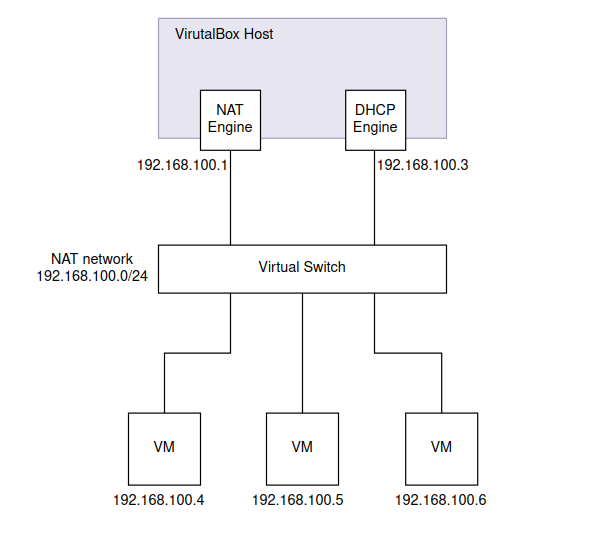
\includegraphics[width=0.5\textwidth]{dev.png}
\caption{Development Enviornment Architecture}
\label{fig:sandbox}
\end{figure}

Regarding Wireguard, virtual machines can be perceived as protocol peers. As the hosts can communicate between themselves, we have a scenario where Wireguard tunnels can be setup. Although in Tailscale's scope Wireguard is considerably abstracted, this environment allows not only a better understanding of the underlying dataplane at stake, but also to collect metrics associated with network performance, using open-source tools, such as iperf ~\cite{iperfws}. Tailscale will then be introduced in the environment, with one machine serving as the control plane, or, by Tailscale's terms, the coordination server. Here, devices, users and subnetting configurations will be done. The other two machines will function as Tailscale clients and are orchestrated by the coordination server. Essentially, this first phase serves as an analysis on Tailscale's concepts, configurations and features, which will aid in specifying and understanding the requirements for the Tailscale instance to be deployed in the \acrshort{ua}'s premises. This environment can also eventually be used for the development of client automation mechanisms, which will be discussed further in the next phases.

Once Tailscale has been researched to its most adequated configuration, we proceed to the next phase, which, analogous to the previous one, consists in the setup of the coordination server in a host within the \acrshort{ua} network, followed by the configuration of the clients, either using the robots running \acrshort{ros} or, in a first stage, a sample of test hosts, which can virtually be any machine.

The final phase consists in the automation of the processes taken in the previous ones, regarding installation, deployment and configuration of both the coordination server and client-side running on the robots. This automation is achieved with the use of shell scripts and, eventually, open-source automation tools such as Ansible ~\cite{ansiblews}. To configure the clients, a config-based script will be developed. This approach allows the use of the same script for all robots requiring access to an overlay network, with a degree of abstraction regarding operations such as key generations and service discovery. Ideally, this script would only require the configuration of the coordination server's address, the name of the network the robot wants to connect to and, optionally, an endpoint pointing to where the robot can be found. Another topic of great interest would be to ensure the robots automatically connect to their desired network on boot, which can be achieved with the use of, for example, crontabs.

The tasks encompassing the phases described above can be summed up in a Gantt diagram, presented in figure \ref{fig:gantt}.

\begin{figure}[h]
\centering
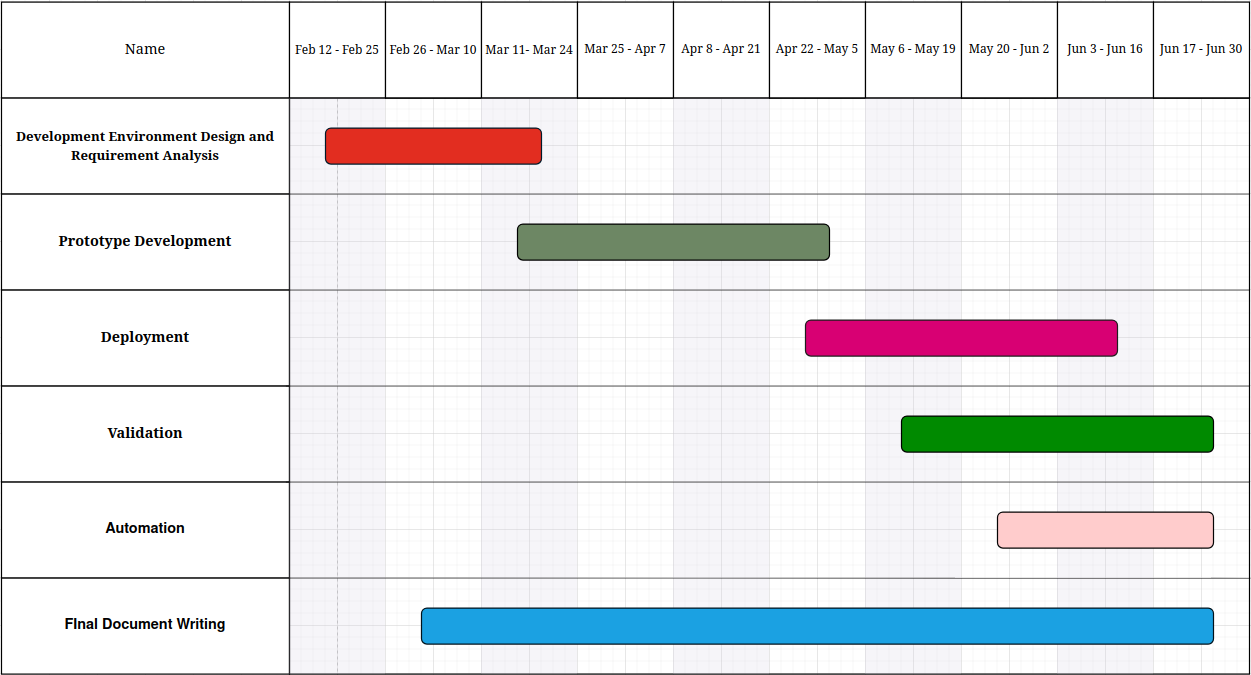
\includegraphics[width=1\textwidth]{gantt.png}
\caption{Development planning proposal}
\label{fig:gantt}
\end{figure}

%
% The bibliography
%
\cleardoublepage
\iffalse
  % Use this is the final version
  %  unsrt produces numbered entries, sorted by order of citation
  %  plain produces numbered entries, sorted alphabetically
  %  other styles are possible (I recommend the harvard package)
  %\bibliographystyle{plain}
  \bibliography{my-bib-file}% replace by the name of name of your .bib file
\else
  % An example (the contents of the .bbl file)
  %\begin{thebibliography}{10}



  %\end{thebibliography}
%\fi

\bibliographystyle{plain}
\bibliography{refs}
\cleardoublepage

\end{document}
